\section{Test and evaluation}

%-----------Without interface--------------------
\subsection{without interface}

\subsubsection{scheduler}
\begin{figure}[H]
    \centering
    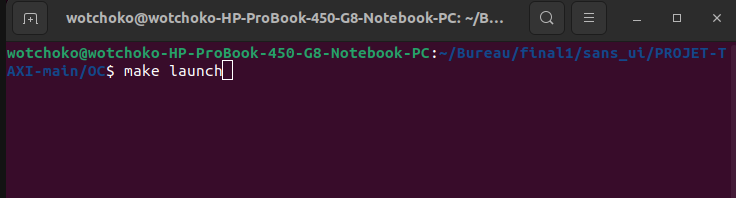
\includegraphics[width=1.0\textwidth]{Sections/Images/new_images/b1.png}
    \caption{compiling scheduler only}
    \label{fig:enter-label}
\end{figure}
\begin{figure}[H]
    \centering
    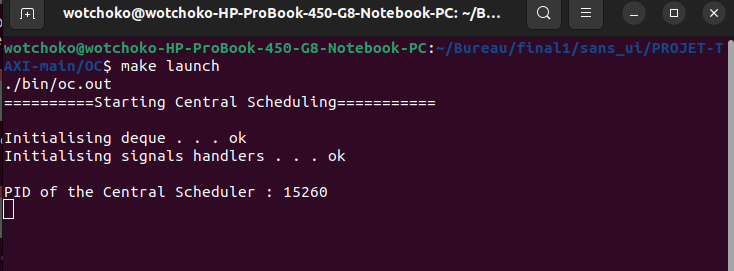
\includegraphics[width=1.0\textwidth]{Sections/Images/new_images/c1.png}
    \caption{result}
    \label{fig:enter-label}
\end{figure}

\begin{figure}[H]
    \centering
    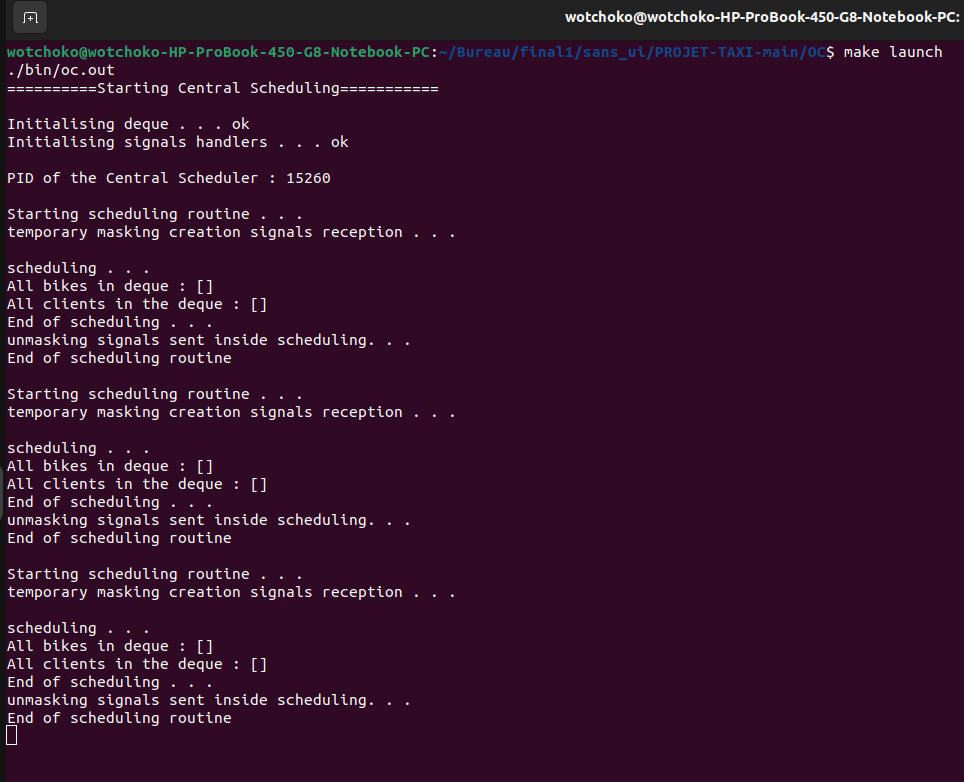
\includegraphics[width=1.0\textwidth]{Sections/Images/new_images/c2.png}
    \caption{we see that deques are empty because clients and bikes are not created.Now we are going to compile it with RPG}
    \label{fig:enter-label}
\end{figure}
\subsubsection{scheduler with RPG}

\begin{figure}[H]
    \centering
    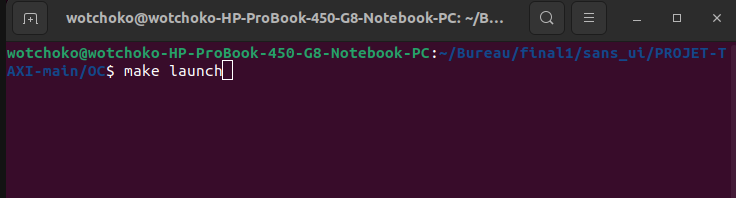
\includegraphics[width=1.0\textwidth]{Sections/Images/new_images/b1.png}
    \caption{to compile OC again}
    \label{fig:enter-label}
\end{figure}

\begin{figure}[H]
    \centering
    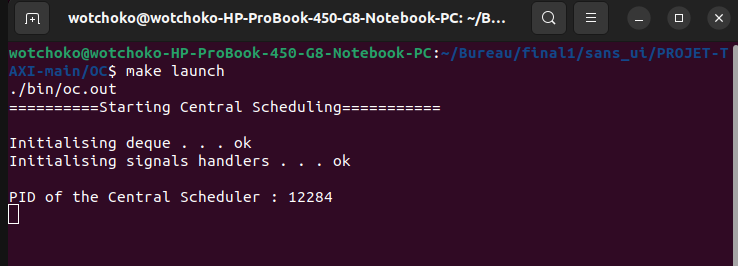
\includegraphics[width=1.0\textwidth]{Sections/Images/new_images/b2.png}
    \caption{new result before RPG}
    \label{fig:enter-label}
\end{figure}

\begin{figure}[H]
    \centering
    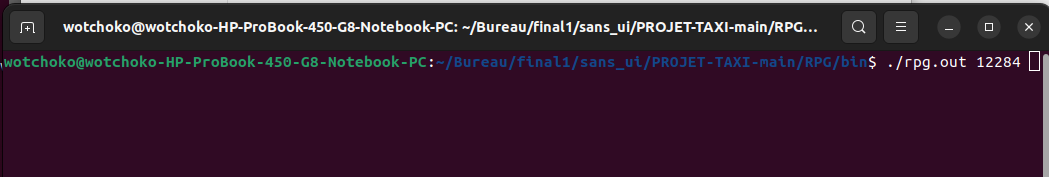
\includegraphics[width=1.0\textwidth]{Sections/Images/new_images/b3.png}
    \caption{to compile RPG with pid of scheduler}
    \label{fig:enter-label}
\end{figure}

\begin{figure}[H]
    \centering
    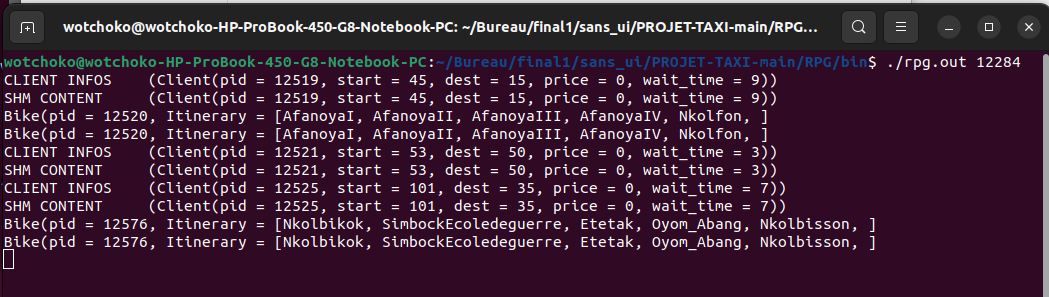
\includegraphics[width=1.0\textwidth]{Sections/Images/new_images/b4.png}
    \caption{result in RPG}
    \label{fig:enter-label}
\end{figure}
% \begin{figure}[H]
%     \centering
%     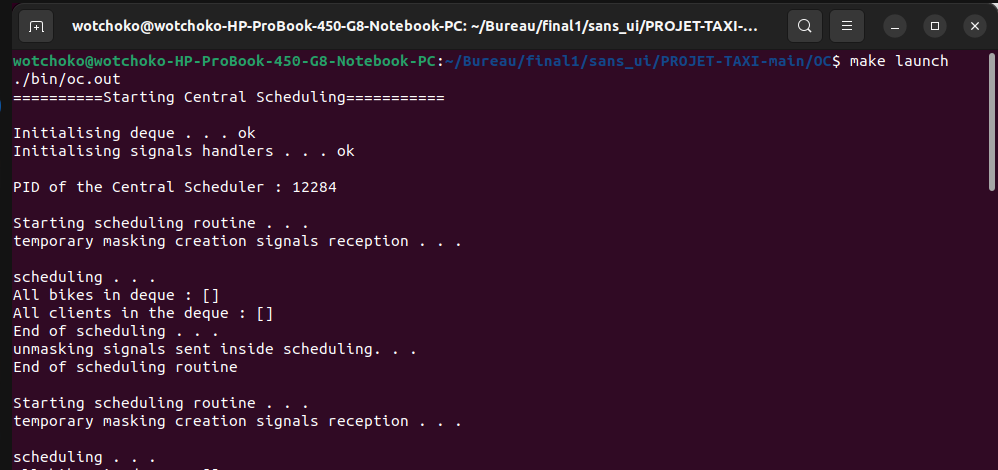
\includegraphics[width=1.0\textwidth]{Sections/Images/new_images/b5.png}
%     \caption{result in RPG}
%     \label{fig:enter-label}
% \end{figure}

\begin{figure}[H]
    \centering
    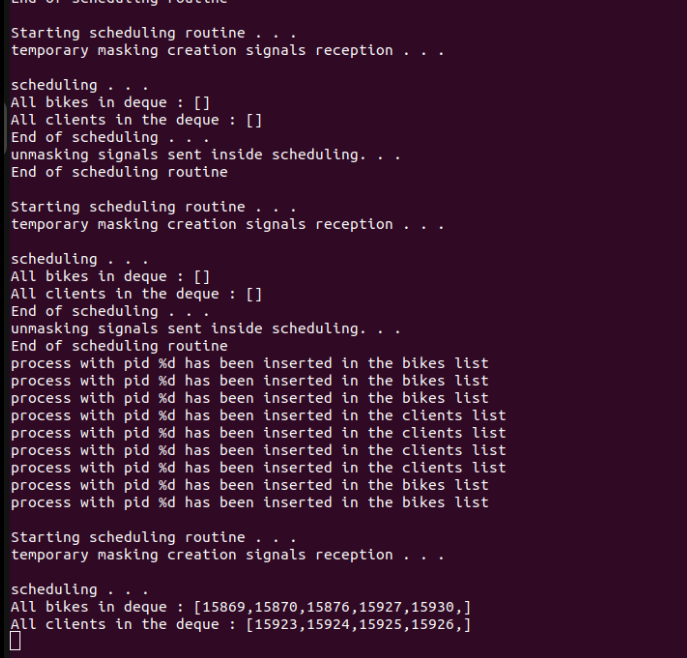
\includegraphics[width=1.0\textwidth]{Sections/Images/new_images/b66.png}
    \caption{scheduling}
    \label{fig:enter-label}
\end{figure}










%-----------With interface-------------

\subsection{with interface}

\begin{figure}[H]
    \centering
    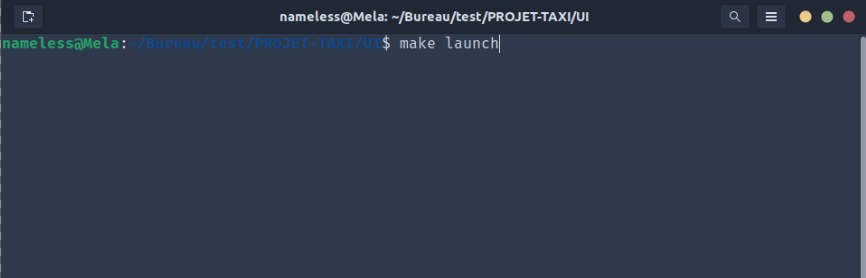
\includegraphics[width=1.0\textwidth]{Sections/Images/new_images/a100.png}
    \caption{compiling of UI}
    \label{fig:enter-label}
\end{figure}

\begin{figure}[H]
    \centering
    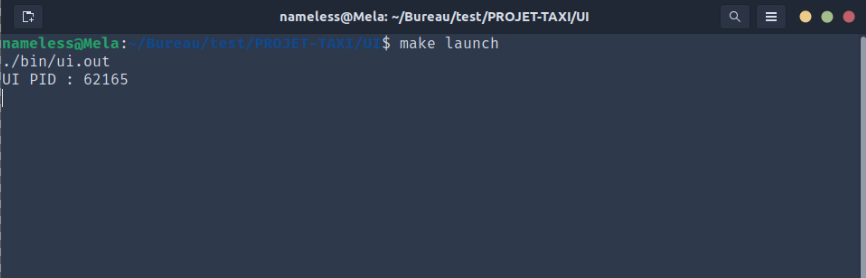
\includegraphics[width=1.0\textwidth]{Sections/Images/new_images/a200.png}
    \caption{result of compiling UI in terminal }
    \label{fig:enter-label}
\end{figure}
\begin{figure}[H]
    \centering
    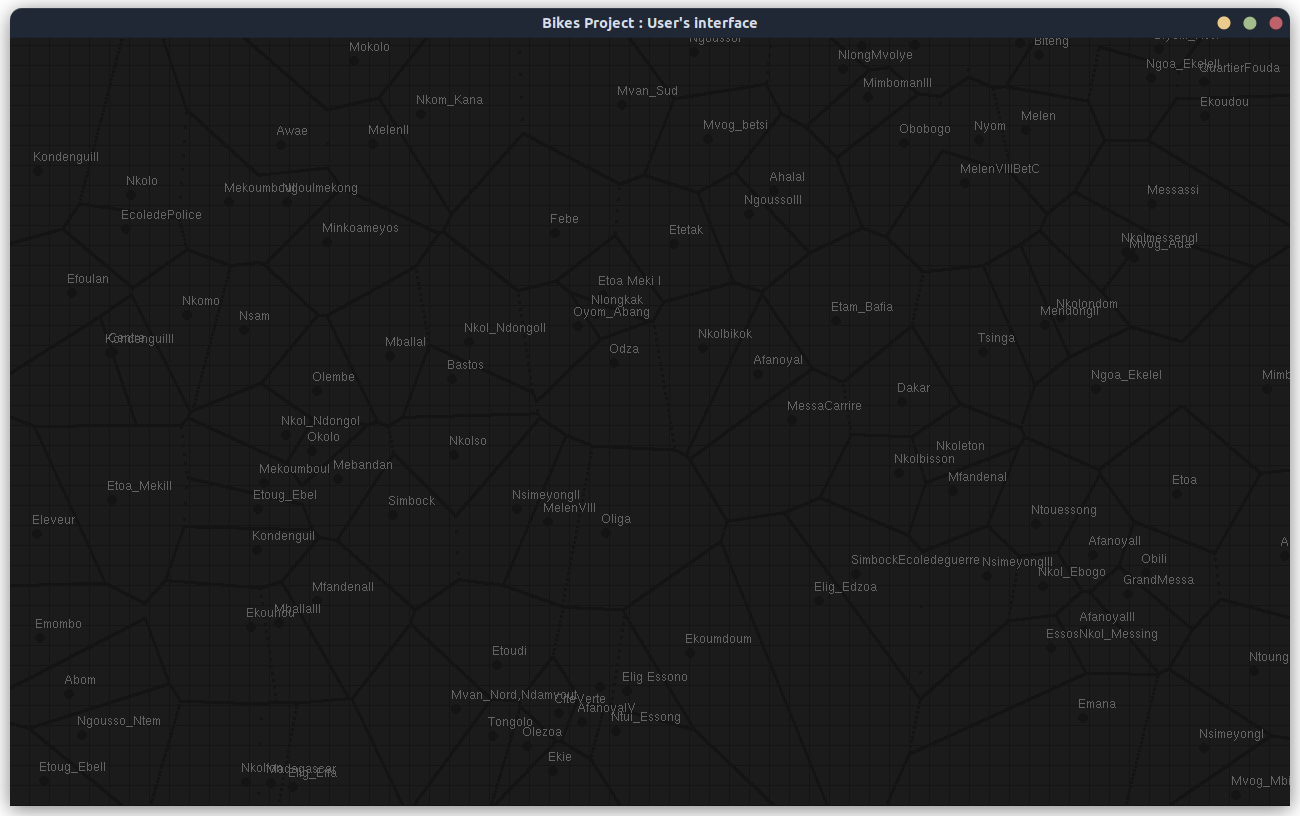
\includegraphics[width=1.0\textwidth]{Sections/Images/new_images/a3.png}
    \caption{result of compiling UI}
    \label{fig:enter-label}
\end{figure}

% \begin{figure}[H]
%     \centering
%     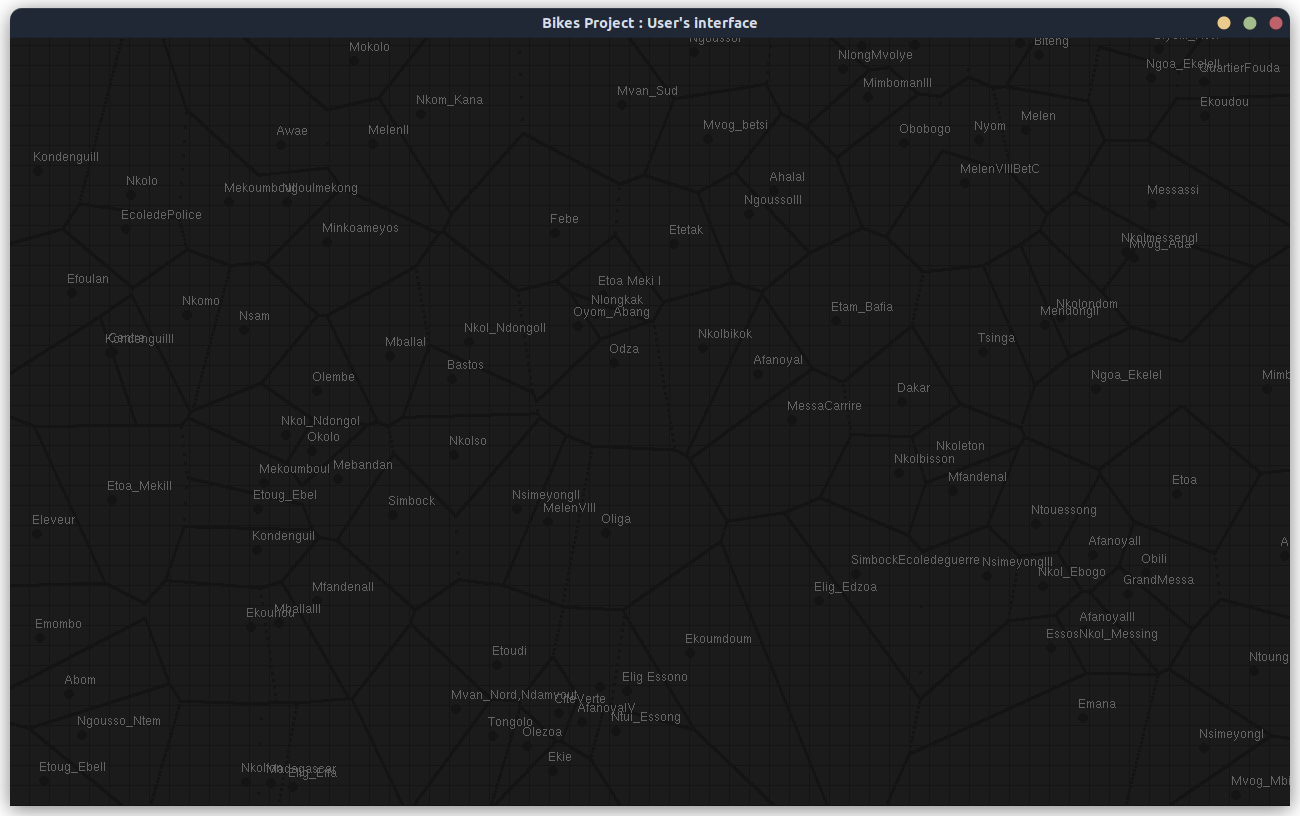
\includegraphics[width=1.0\textwidth]{Sections/Images/new_images/a3.png}
%     \caption{compiling of OC with the pid of UI}
%     \label{fig:enter-label}
% \end{figure}

\begin{figure}[H]
    \centering
    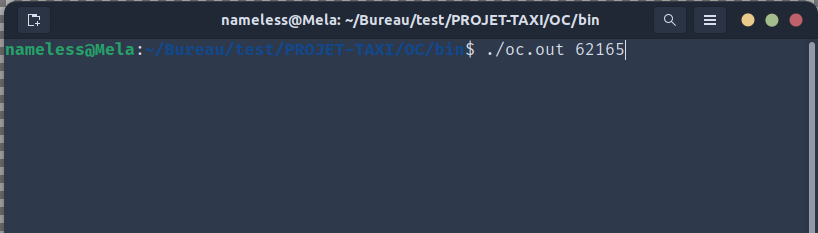
\includegraphics[width=1.0\textwidth]{Sections/Images/new_images/a400.png}
    \caption{compiling OC with pid of UI}
    \label{fig:enter-label}
\end{figure}

\begin{figure}[H]
    \centering
    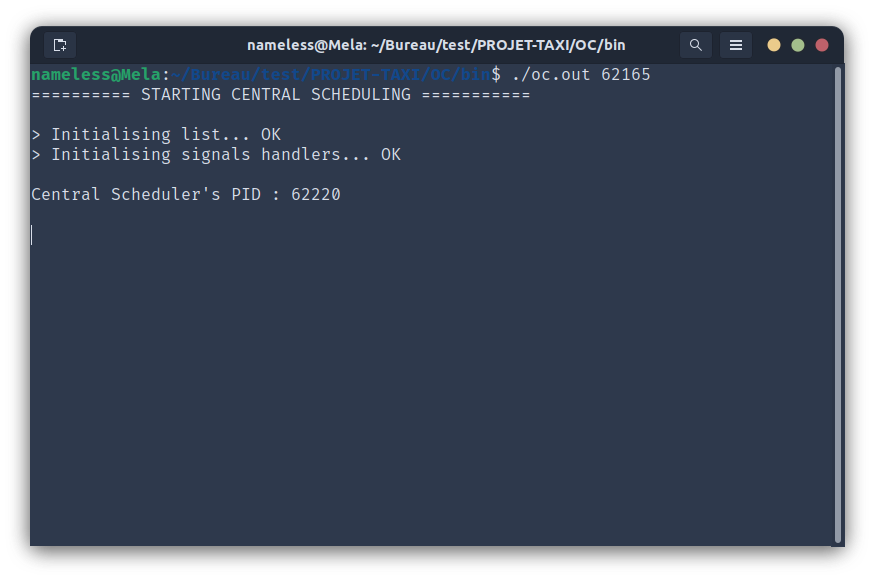
\includegraphics[width=1.0\textwidth]{Sections/Images/new_images/a5.png}
    \caption{result before the compilation of RPG}
    \label{fig:enter-label}
\end{figure}

\begin{figure}[H]
    \centering
    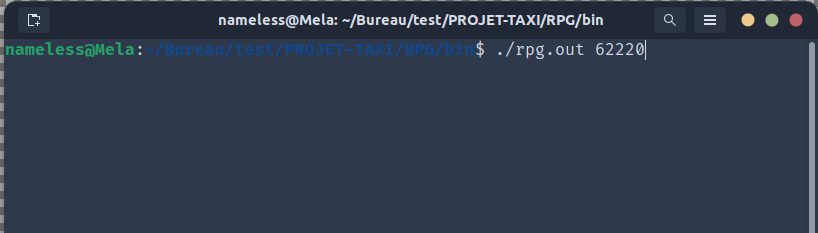
\includegraphics[width=1.0\textwidth]{Sections/Images/new_images/a600.png}
    \caption{compiling RPG with pid of OC}
    \label{fig:enter-label}
\end{figure}

% \begin{figure}[H]
%     \centering
%     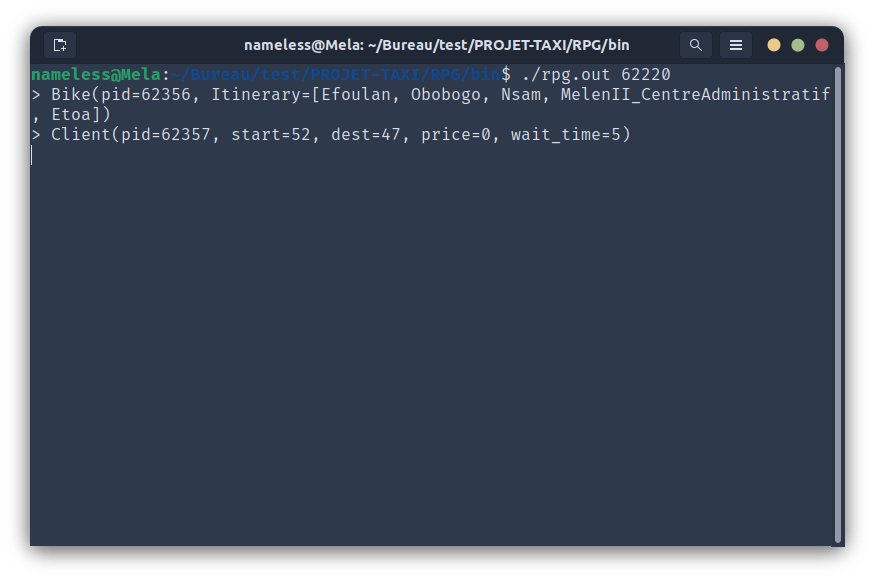
\includegraphics[width=1.0\textwidth]{Sections/Images/new_images/a7.png}
%     \caption{OC result}
%     \label{fig:enter-label}
% \end{figure}

\begin{figure}[H]
    \centering
    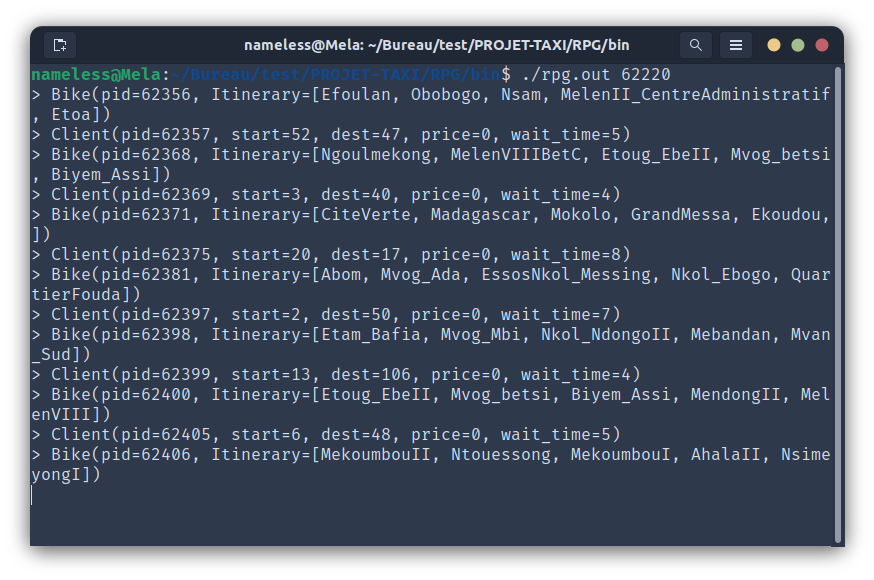
\includegraphics[width=1.0\textwidth]{Sections/Images/new_images/a8.png}
    \caption{RPG result}
    \label{fig:enter-label}
\end{figure}

\begin{figure}[H]
    \centering
    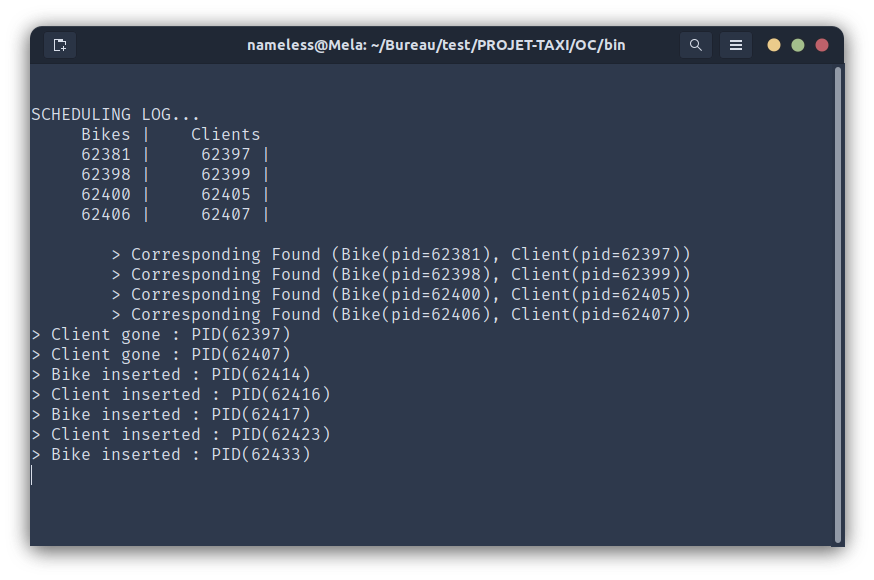
\includegraphics[width=1.0\textwidth]{Sections/Images/new_images/a9.png}
    \caption{OC result}
    \label{fig:enter-label}
\end{figure}

\begin{figure}[H]
    \centering
    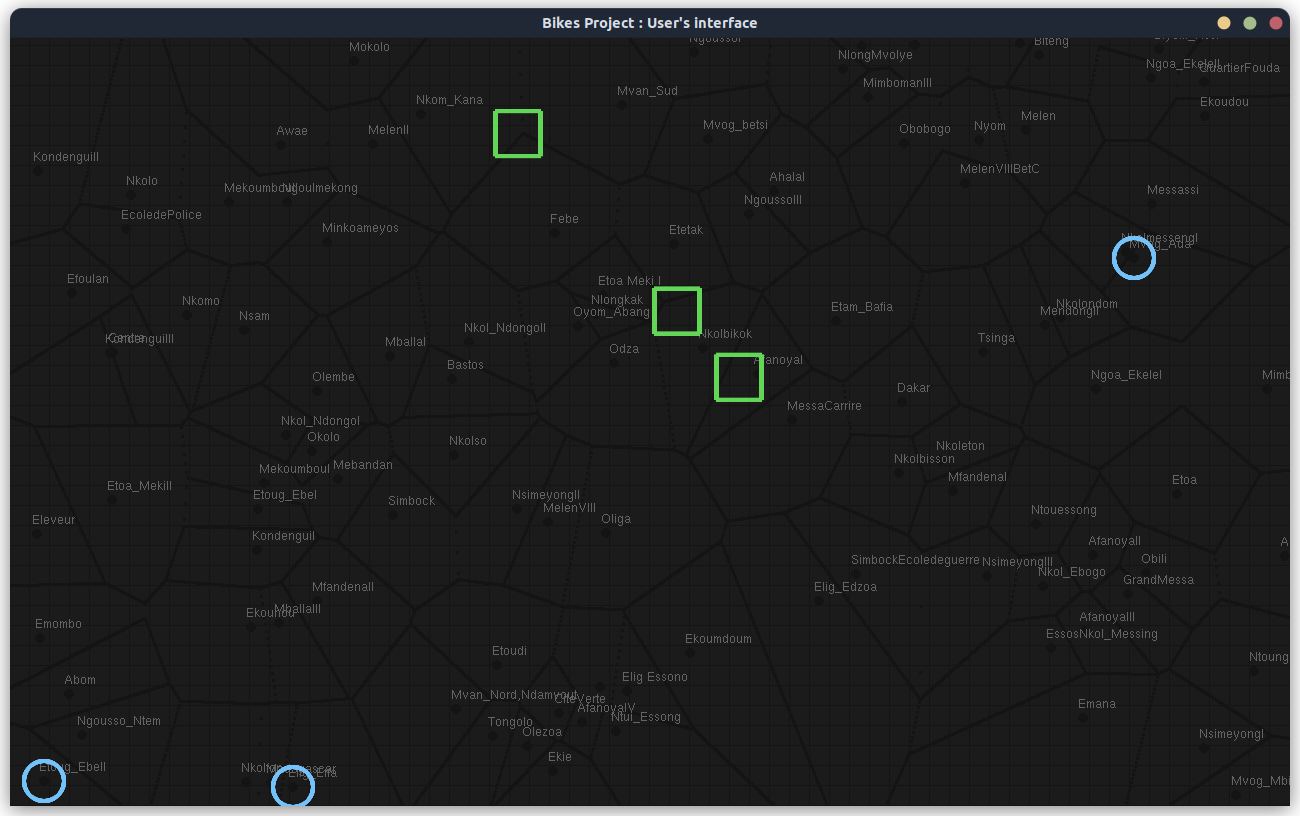
\includegraphics[width=1.0\textwidth]{Sections/Images/new_images/a10.png}
    \caption{interface result}
    \label{fig:enter-label}
\end{figure}

\begin{figure}[H]
    \centering
    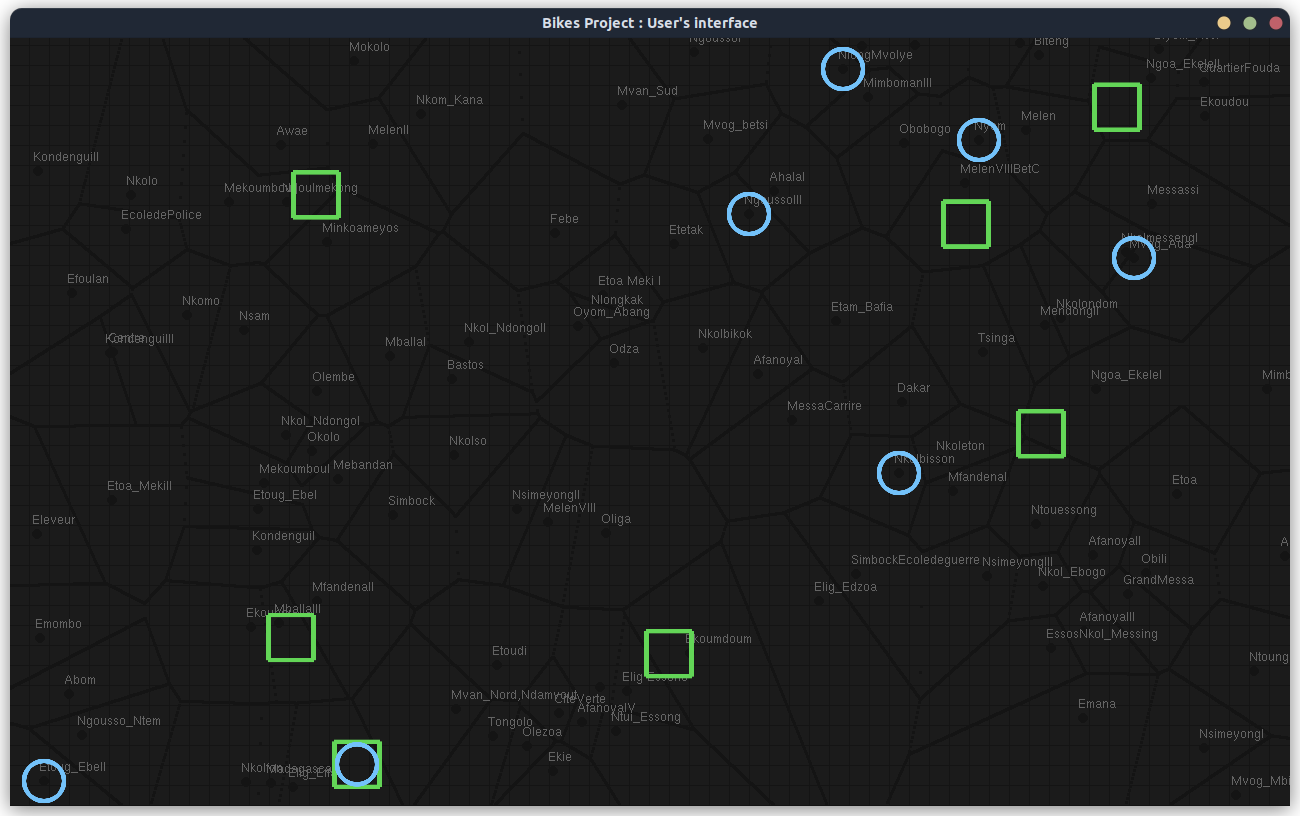
\includegraphics[width=1.0\textwidth]{Sections/Images/new_images/a11.png}
    \caption{interface result}
    \label{fig:enter-label}
\end{figure}

\begin{figure}[H]
    \centering
    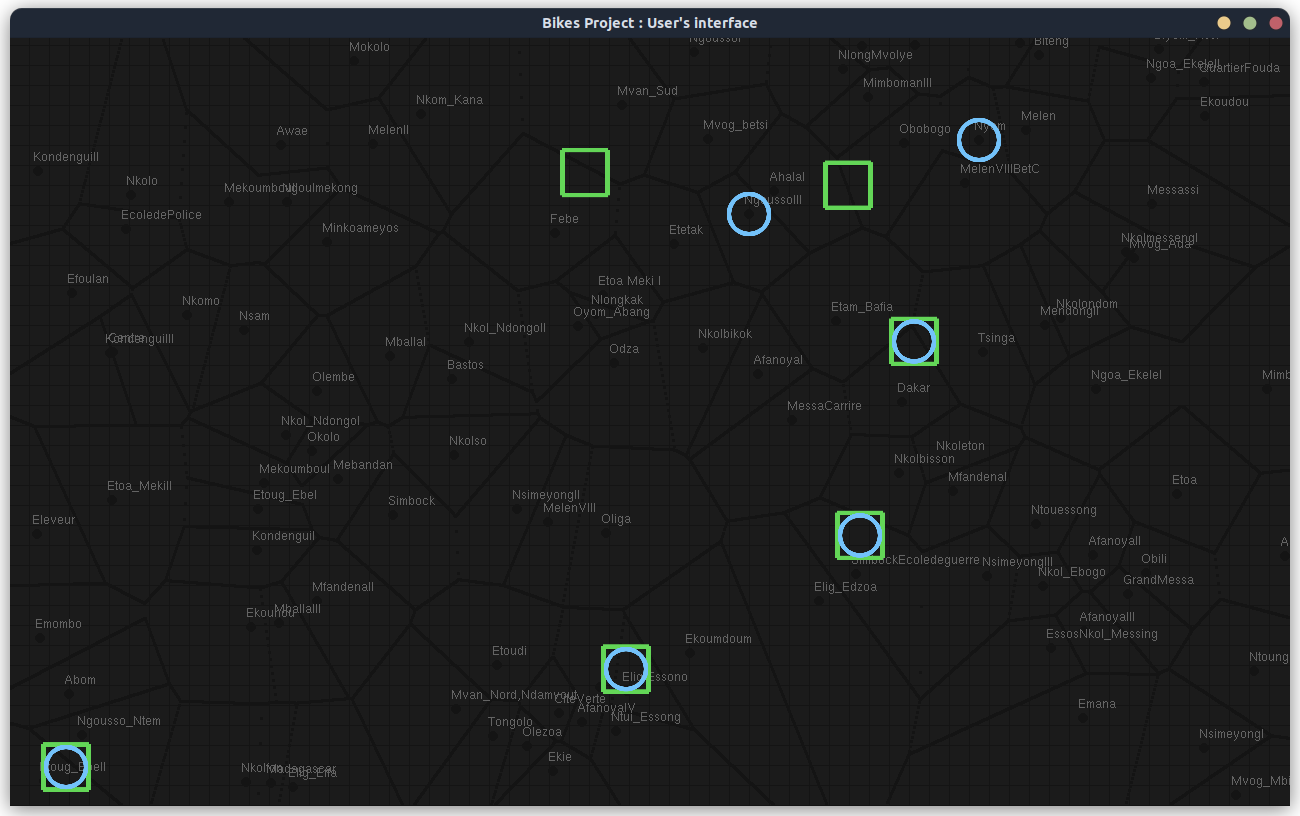
\includegraphics[width=1.0\textwidth]{Sections/Images/new_images/a12.png}
    \caption{interface result}
    \label{fig:enter-label}
\end{figure}

\begin{figure}[H]
    \centering
    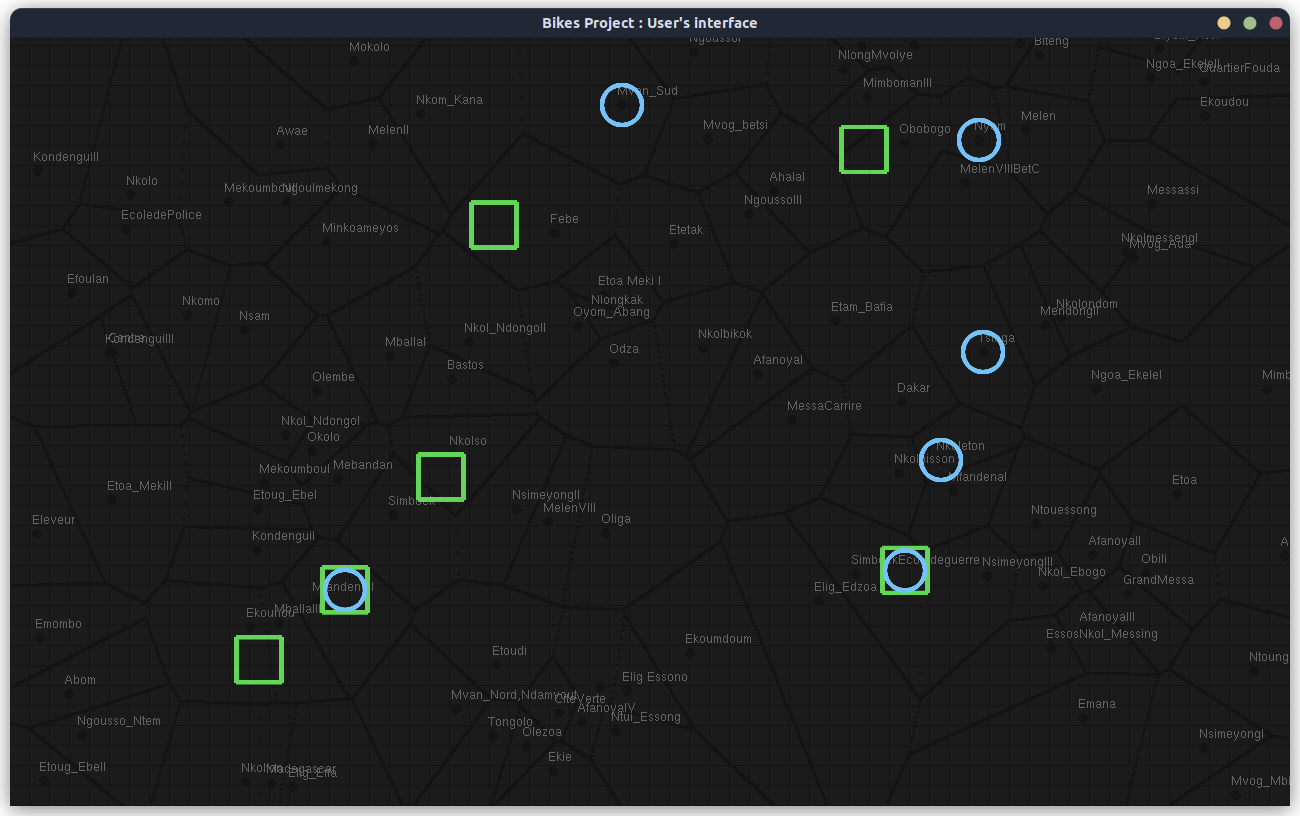
\includegraphics[width=1.0\textwidth]{Sections/Images/new_images/a13.png}
    \caption{interface result}
    \label{fig:enter-label}
\end{figure}
